\documentclass[a4paper]{report}
\usepackage{graphicx}
\usepackage{array}
\usepackage{natbib}
\usepackage{hyperref}
\usepackage[english]{babel}
\usepackage{lscape}
\usepackage{longtable}

\begin{document}
\begin{titlepage}
\begin{center}
\textsc{\LARGE Contextproject Programming Life}\\
\vspace{5pt}
\textsc{\LARGE Group 2 - GEVATT}\\
\vspace{5pt}
\textsc{\LARGE Final Report}\\
\vspace{5pt}
\textsc{\large TU Delft}

\begin{table}[ht]
\centering
\begin{tabular}{ccc}

\includegraphics[scale=0.2]{ruben.png}   &

\includegraphics[scale=0.2]{mathijs.png} &

\includegraphics[scale=0.2]{jasper.png}  \\
Ruben Bes	& Mathijs Hoogland	& Jasper Denkers\\
rbes 		& mhhoogland 		& jdenkers\\
4227492 	& 4237676 			& 4212584\\
\end{tabular}
\end{table}

\begin{table}[ht]
\centering
\begin{tabular}{cc}
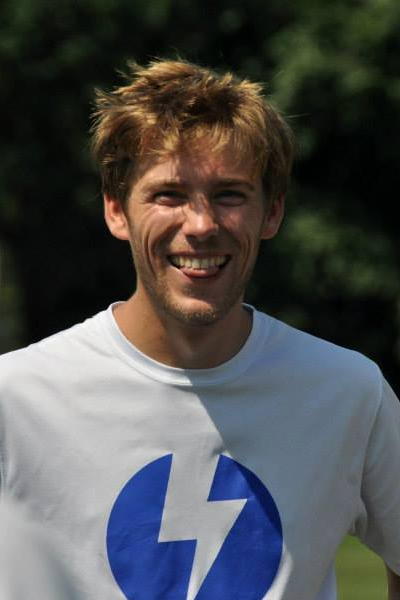
\includegraphics[scale=0.2]{robbert.png} &

\includegraphics[scale=0.2]{willem.png}  \\
Robbert van Staveren	& Willem Jan Glerum\\
rhvanstaveren 			& wglerum\\
1527118					& 4141040\\
\end{tabular}
\end{table}

\vfill
{\large \today}
\end{center}

\end{titlepage}

\begin{landscape}
\setlength\extrarowheight{5pt}
\begin{longtable}{p{3cm}|p{5cm}|l|l|l|l|p{7cm}}

\textbf{Story} & \textbf{Task} & \textbf{Effort} & \textbf{Assignment} & \textbf{Actual effort} & \textbf{Done} & \textbf{Notes}\\
\hline \hline

A user wants to have an overview of mutations per patient & Look for homozygoot mutations & 4 & Mathijs & & &\\
& Look up the exact definition of CADD score and look if the score of 0 can be avoided & 4 & & & &\\
& Implement the XY/XX chromosome & 10 & & & &\\
\hline

A user wants to view links between genes and proteins related to a mutation & Protein visualization per node in the mutation view & 4 & Jasper & & &\\
& Link deseases to genes & 4 & Ruben & 3 hours & Yes & Had to make a few getters and setters and perform shotgun surgery\\
& Show multiple mutations per graph & 6 & & & &\\
& Extend the the proteine graph & 6 & Robert & & &\\
& And make them clickable & 2 & & & &\\
\hline

A user looks at an overview of the location of a mutation & Link Ensemble ID to String database & 4 & Willem Jan & & &\\
& Store GTF information in database & 4 & & & &\\
& Look if other genes are near the starting point of a mutation & 6 & & & &\\
& Show neighbouring mutations & 6 & & & &\\
\hline

Database testing & Test database, mocking doesn't work, use a test database & 8 & & & &\\
& Give proper errors when database fails & 4 & & & &\\
\hline

A user logs in and views basic information & Optimize dashboard information & 2 & & & &\\
& Make breadcrumbs on each page & 2 & & & &\\
\hline

Deliverables & Scrum plan 4 week 7 & 1 & Willem Jan & & &\\
& Scrum reflection 4 week 7 & 2 & & & &\\
& Final Report Draft & 8 & & & &\\
& Architecture Design Draft & 4 & & & &\\
\hline
\end{longtable}
\end{landscape}

\section*{General Reflection}

\end{document}